\chapter{Resultados}\label{cap:resultados}
\section{Introdução}

Os dados de temperatura coletados foram salvos em um arquivo csv, testados com o algoritmo de intervalo de confiança móvel ajustado para avaliar o dado em uma amostra dos últimos 10 valores. 
Na tabela~\ref{tab:tamanhovetor} mostra a quantidade de dados que foram considerados validos em comparação a quantidade de últimas amostras coletadas, o algoritmo visa rodar em ambiente embarcado limitado onde quantidade de memoria e processamento são escassos, com isso o tamanho do vetor pode ser uma variável significativa na tomada de decisão. O vetor escolhido apresenta 10 casas de amostra e suas características foram descritas logo em seguida.

\begin{longtable}{|p{4cm}|p{3.5cm}|}
    \hiderowcolors
    \caption{Tamanho do vetor de amostra versus quantidade de dados filtrados}
    \label{tab:tamanhovetor}\\
    \showrowcolors
    \hline
    \rowcolor[HTML]{C0C0C0} 
    \multicolumn{1}{c|}{\cellcolor[HTML]{C0C0C0}\textbf{TAMANHO}} & \multicolumn{1}{c|}{\cellcolor[HTML]{C0C0C0}\textbf{DADOS FILTRADOS}} \\ \hline

    \endfirsthead
    \rowcolor[HTML]{C0C0C0} 
    \multicolumn{1}{c|}{\cellcolor[HTML]{C0C0C0}\textbf{TAMANHO}} & \multicolumn{1}{c|}{\cellcolor[HTML]{C0C0C0}\textbf{DADOS FILTRADOS}} \\ \hline

    \endhead
		\hline
		5	& 619	\\
		\hline
		10	& 404	\\
		\hline
		20	& 371	\\
		\hline
		30	& 383	\\
		\hline
		40	& 393	\\
		\hline
		50	& 385	\\
		\hline
		60	& 343	\\
		\hline
		70	& 296	\\
		\hline
		80	& 277	\\
		\hline
		90	& 266	\\
		\hline
		100	& 261	\\
		\hline
		200	& 391	\\
		\hline
    
    \end{longtable}

E importante ressaltar que em ambiente de sistema embarcado, a quantidade de memoria disponível para armazenar um vetor com muitas posições e pequena. Com isso, se torna um ponto positivo o sistema que consiga entregar uma filtragem aceitável com pouca alocação de memoria. 

% Os resultados podem ser visualizados na Figura~\ref{fig: Cleaning_sensor_data_overlay_visualization}, onde os pontos verdes significam que foram coletados e os em vermelhos foram ignorados. Já no gráfico ..
Na Figura~\ref{fig: graficos_tamanhos_amostras} podemos visualizar como o algoritmo se comporta de acordo com o tamanho do vetor de amostras, percebe-se que quanto maior o vetor menor a taxa de dados que passam pelo filtro, também presenciamos uma pior leitura nos picos de sinais já que o mesmo só começa a considerar os valores validos quando a curva já está em queda. O vetor com 5 amostra tem um período menor para considerar os novos valores, com isso muitos dos valores foram considerados limpos, isso pode ser bom visando que o tempo de coleta seja curto, mas em casos que deseja-se uma maior precisão um período maior de coleta parece ser mais adequado. 


\begin{figure}[H]
	\centering
	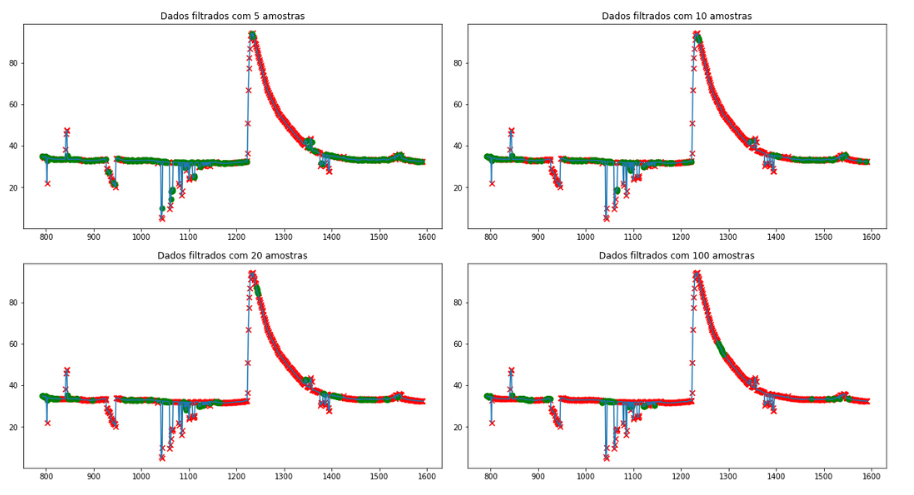
\includegraphics[width=15cm]{imagens/sensores/graficos_tamanhos_amostras.jpg}
	\caption{Gráficos mostrando a relação de tamanho da amostra versos quantidade de dados filtrados}
	Fonte: Autor
	\label{fig: graficos_tamanhos_amostras}
\end{figure}

Com 10 valores percebe-se que o algoritmo consegue pegar bem a ponta dos picos de temperatura, ignorando muitos dos ruídos mas com uma boa taxa de validação de dados, por isso levamos em consideração essa quantidade de amostras no teste, mas vale lembrar que essa quantidade pode e deve ser customizada de acordo com o problema, limitações e tempo em que a aplicação ira existir.

Nota-se a dificuldade do algoritmo em considerar os dados que estão em uma curva ascendente ou decrescente, mas destacam-se por conseguir capturar os dados da ponta de todos os grandes picos de sinal, em todos dos casos o tempo em que se levou para uma nova coleta depois de uma queda ou subida brusca e considerável, deixando claro que em caso de uma curva muito longa o programa pode travar esperando uma resposta, por isso e de importância avaliar se deve haver um controle de chamada do valor mesmo que esteja fora do intervalo mas com um tempo já decorrido consideravelmente.


\begin{figure}[H]
	\centering
	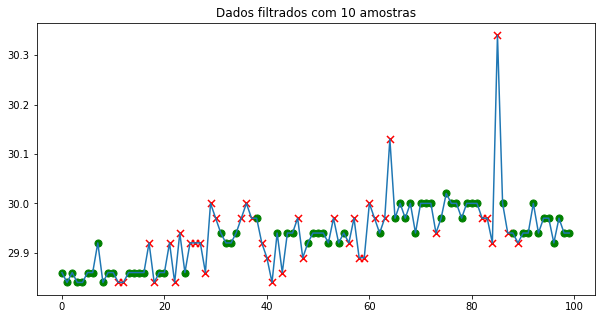
\includegraphics[width=15cm]{imagens/sensores/filtrado_100_ultimas.png}
	\caption{Dados de 1530 a 1590}
	Fonte: Autor
	\label{fig: indice}
\end{figure}

No trecho da figura~\ref{fig: indice} temos o trecho das primeiras 100 linhas, podemos notar como o algoritmo coleta os dados de forma precisa por mais que o desvio dos valores não seja grande, esses dados podem ser tratados posteriormente com uma simples média móvel ou outra função de preferencia.


\begin{figure}[H]
	\centering
	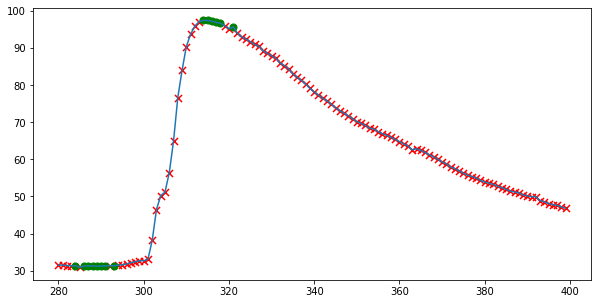
\includegraphics[width=15cm]{imagens/sensores/indice2.png}
	\caption{Curva de temperatura no trecho de 280 a 400}
	Fonte: Autor
	\label{fig: indice2}
\end{figure}

Na Figura~\ref{fig: indice2} o programa mostra sua falha em capturar curvas expressivas de dados, conseguindo capturar os valores do topo mas ignorando grande parte dos valores. Essa característica indesejável não parece ser corrigida com nenhum tamanho de amostra utilizado aqui neste trabalho, com todas falhando em lidar com sinuosidades.

\begin{figure}[H]
	\centering
	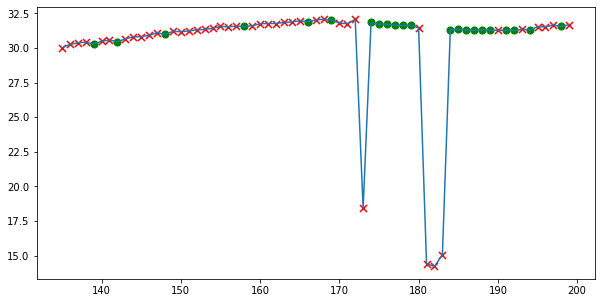
\includegraphics[width=15cm]{imagens/sensores/indice4.png}
	\caption{Conjunto de dados de 130 a 200}
	Fonte: Autor
	\label{fig: indice4}
\end{figure}

Na Figura~\ref{fig: indice4} podemos visualizar bem alguns ruídos que se destacam dos dados originais e como o algoritmo se comporta na sua filtragem, os valores que chegam a ter \ang{17}c de diferença são descartados já que apresentam características de ruído pela sua dessemelhança em tão pouco tempo.

\begin{figure}[H]
	\centering
	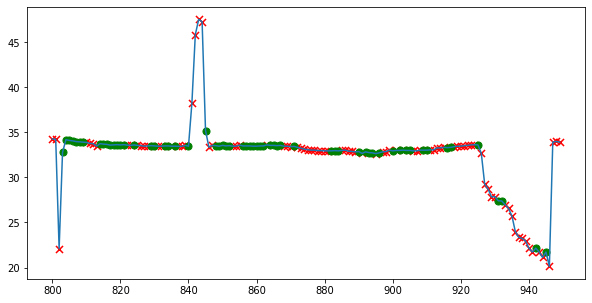
\includegraphics[width=15cm]{imagens/sensores/indice3.png}
	\caption{Dados de 800 a 950}
	Fonte: Autor
	\label{fig: indice3}
\end{figure}

Já na Figura~\ref{fig: indice3} presenciamos ruídos discrepantes de forma muito negativa e muito positiva, nota-se que os dados de 920 a 950 podem ser considerados ruídos pelo seu curto espaço de tempo, mas pela quantidade de amostra ser pequena alguns dos valores entraram como verdadeiros, enfatizando ainda mais que o tamanho do vetor de amostra deve ser dimensionado de acordo com os propósitos de precisão da aplicação.

Durante a execução do algoritmo notou-se o problema de laço teoricamente infinito caso não seja encontrado um valor dentro do intervalo de confiança, esse tempo pode ser prejudicial ou não dependendo da aplicação, então aconselha-se que seja definido um tempo limite para coleta do dado mesmo que esteja fora do intervalo de confiança. 

\begin{algorithm}[H]
    \Entrada{Tamanho do vetor de amostras ($TV$), Vetor de amostras ($VA$), Tempo limite de tentativas ($T$)}
    \Saida{Valor considerado verdadeiro ($resultado$), Vetor de amostras ($VA$)}
    \Inicio{
		\While{$resultado == SemValor$}{

			$V \leftarrow coletaDadoDoSensor()$; \tcc*[f]{Coleta dado do sensor} \\

			\Se{$T \leq 0$}{ 
				$resultado \leftarrow V$;
			}
			$T \rightarrow 1$;  \tcc*[f]{Decrementa tempo} \\

			\Se{$tamanho(VA) \geq TV$}{ 

				$primeiroIntervalo$, $segundoIntervalo \leftarrow intervaloDeConfianca($VA$)$; 

				\Se{$V \geq primeiroIntervalo$ \&\& $V \leq segundoIntervalo$}{
					$resultado \leftarrow V$; 
				}
				
				$VA \rightarrow primeiroElemento$; \tcc*[f]{Remove elemento mais velho} \\
			}

			$VA \leftarrow V$; \tcc*[f]{Adiciona valor para dentro do vetor de amostra} \\
		}


		\tcc*[f]{Retorna valor verdadeiro e vetor com as ultimas amostras} \\
		\Retorna $resultado$, $VA$; 
    }
    \caption{Algoritmo que considera o tempo na coleta do sensor}
    \label{algoritmo:alg_com_temp}
\end{algorithm}

Principalmente em ambiente embarcado, onde as rotinas de interrupção podem interromper a leitura do sensor em um tempo critico, ou as rotinas de seguranças podem reiniciar o sistema por culpa da característica de loop infinito ou de bloqueio do sistema advindo da função utilizada.